%% ICFNDS 2026 — IoT Track
%% For blind review (CHECK THE PORTAL FIRST — ICFNDS has historically been non-blind):
%%   \documentclass[sigconf,anonymous,review]{acmart}
\documentclass[sigconf]{acmart}

\usepackage{booktabs}
\usepackage{graphicx}
\usepackage{amsmath}
\usepackage{subcaption}
\usepackage{seqsplit}

%% --- Publication metadata -------------------------------------------------
%% TODO: replace with the exact strings from the ICFNDS camera-ready instructions.
%% Do not guess the edition number of the conference.
\copyrightyear{2026}
\acmYear{2026}
\setcopyright{acmlicensed}
\acmConference[ICFNDS 2026]{International Conference on Future Networks and
  Distributed Systems}{November 04--06, 2026}{İzmir, Türkiye}
\acmISBN{978-x-xxxx-xxxx-x/26/11}   % TODO
\acmDOI{10.1145/nnnnnnn.nnnnnnn}    % TODO

\begin{document}

%% TODO: pick per the decision rule in docs/DECISION_RULES.md.
%% Branch (a): "Tokens That Persist: ..."   Branches (b)/(c): "Does Identity Persistence Matter? ..."
\title{Tokens That Persist: Entity-Centric Video Tokenization for Group
  Engagement Analysis at the Edge}
%% TODO before submission: repo push status is unverified -- this project's
%% earlier attempt to push to this remote hit an unresolved 403
%% permission-denied error, and the working tree is currently 13 commits
%% ahead of origin/main with nothing pushed this session. Confirm the repo
%% is actually public and up to date at this URL before relying on this note,
%% and confirm anonymous-review requirements don't prohibit an identifying
%% URL before this note ships in a submitted (as opposed to camera-ready) copy.
\titlenote{Code, configs, and decision-rule logs:
  \url{https://github.com/multi-modal-rtm/ept}}

\author{Abdulaziz Xo'jamqulov}
\affiliation{%
  \institution{Tashkent University of Information Technologies}
  \city{Tashkent}
  \country{Uzbekistan}}
\email{}

%% TODO: confirm the author list and order with all coauthors before submission.

\begin{abstract}
A patch token in a video transformer has no persistent referent: the same
spatial cell at time $t$ and $t{+}1$ denotes the same physical content only
by accident. We test whether restoring persistence --- one token per tracked
entity per time segment, rather than one token per spatial cell --- changes
what a video transformer learns, using an identity-shuffle control that
holds entity localization, token count, and architecture fixed and varies
only whether the same entity occupies the same token slot across segments.
Under a decision rule and effect-size floor frozen before any test-split
evaluation, three pre-registered structural hypotheses --- persistence on a
multi-party dialogue benchmark (MELD), entity structure on the same
benchmark, and entity structure's replication on a single-subject webcam
benchmark (DAiSEE) --- are all null: two are positive but underpowered by
the pre-registered floor, one is indistinguishable from zero outright. We
report entity-localized tokenization's compute cost separately from these
outcomes: encoder cost falls $4.53\times$ relative to a matched-budget
spatial grid, the architecture's own attention stays under $0.03\%$ of total
per-clip compute across every condition and budget-sweep cell tested, and
end-to-end cost including detection --- measured
across three internally consistent hardware regimes after a GPU detection
path could not be made to work --- ranges from $0.23\times$ to $7.49\times$
a grid baseline depending on where detection runs. A byproduct of preparing
this evaluation was discovering and diagnosing severe train/test leakage in
the classroom-engagement benchmark originally intended as primary; we report
that finding and the reusable admission procedure it produced alongside the
null hypothesis results.
\end{abstract}

%% TODO before submission: the five concept_id numbers below are NOT independently
%% verified against ACM's live CCS tool -- https://dl.acm.org/ccs.cfm returned 403
%% (blocked) and dlccsdev.acm.org did not resolve, in every attempt made this
%% session. "Activity recognition and understanding"'s ID was corrected once already
%% after a web search surfaced a real paper using a longer, different ID than the
%% first guess (...10010225 -> ...10010225.10010228); the same could be true of any
%% of the other four, which were not independently cross-checked against a real
%% paper's source the way that one was. Regenerate this whole block from the live
%% tool before camera-ready -- do not trust these numbers as final.
\begin{CCSXML}
<ccs2012>
   <concept>
       <concept_id>10010147.10010178.10010224.10010225.10010228</concept_id>
       <concept_desc>Computing methodologies~Activity recognition and understanding</concept_desc>
       <concept_significance>500</concept_significance>
       </concept>
   <concept>
       <concept_id>10002944.10011122.10002945</concept_id>
       <concept_desc>General and reference~Evaluation</concept_desc>
       <concept_significance>300</concept_significance>
       </concept>
   <concept>
       <concept_id>10010147.10010257.10010293.10010294</concept_id>
       <concept_desc>Computing methodologies~Neural networks</concept_desc>
       <concept_significance>300</concept_significance>
       </concept>
   <concept>
       <concept_id>10002944.10011122.10002947</concept_id>
       <concept_desc>General and reference~Measurement</concept_desc>
       <concept_significance>100</concept_significance>
       </concept>
   <concept>
       <concept_id>10010583.10010584</concept_id>
       <concept_desc>Computer systems organization~Embedded systems</concept_desc>
       <concept_significance>100</concept_significance>
       </concept>
 </ccs2012>
\end{CCSXML}

\ccsdesc[500]{Computing methodologies~Activity recognition and understanding}
\ccsdesc[300]{General and reference~Evaluation}
\ccsdesc[300]{Computing methodologies~Neural networks}
\ccsdesc[100]{General and reference~Measurement}
\ccsdesc[100]{Computer systems organization~Embedded systems}

\keywords{video understanding, tokenization, attention efficiency, engagement
  recognition, edge inference}

\maketitle

\section{Introduction}
%% paper/sections/intro.tex
%% Draft only. No results, no methods, no conclusions -- see
%% docs/DECISION_RULES.md and logs/GATES.md for why those wait.

A text token has a referent that survives its position: the word ``teacher''
at sequence index 3 and the same word at index 40 name the same lexical
item, and a language transformer's attention over those two positions is
answering a well-posed question --- \emph{how related are these two
mentions of the same thing?} A patch token in a video transformer has no
such guarantee. A grid cell at spatial location $(i,j)$ in frame $t$ and the
same cell in frame $t{+}1$ denote the same thing only if nothing has moved
through that cell, an assumption video violates constantly and by design ---
people walk, cameras pan, occlusion happens. Divided space-time and
factorised attention over a fixed patch grid nonetheless price every pairwise
affinity between these positions as if the grid supplied a stable identity
axis. It does not. The tokens are referent-free.

This paper asks a narrow, checkable question that follows from that
observation: does giving a video transformer tokens with a genuine
persistent referent --- one token per tracked entity per time segment,
rather than one token per spatial cell --- change what the model can learn,
and is the effect attributable to \emph{persistence itself} rather than to
two things that usually travel with it, entity-localized cropping (looking
only at where an entity is, instead of the whole frame) and a smaller,
matched token budget? Prior entity- and object-centric video representations
motivate the persistence hypothesis but rarely isolate it from these
confounds (\S\ref{sec:related-work}); we design a control that shuffles
entity identity across time segments while holding architecture, token
count, and every other factor fixed, so that any gap between the shuffled
and unshuffled conditions is attributable to persistence and only to
persistence (\S\ref{sec:method}).

Answering that question honestly turned out to require answering a
prior one first: is the benchmark we asked it on actually testing what it
claims to test? Our first candidate primary dataset, OUC-CGE, a recent
classroom group-engagement corpus~\cite{lu2025ouccge}, failed that check. A
linear probe on a single mean-pooled frame embedding --- no temporal
structure, no entities, no attention, nothing an architecture paper would
want credit for --- reaches
%% outputs/phase3_5_audit/REPORT.md sec.4
macro-F1 $0.9748$ on its provided validation split, statistically
indistinguishable from a full entity-persistent transformer trained on the
same split (
%% outputs/phase3_5_audit/REPORT.md sec.4, citing the locked-recipe A1 result
$0.9767$). The same probe, unchanged, scores
%% outputs/dataset_admission/daisee/admission_report.json: trivial_probe.val_macro_f1
$0.2177$ on DAiSEE~\cite{gupta2016daisee}, a dataset built with a
subject-disjoint split. The gap is not a property of the probe; it is a
property of the split. \S\ref{sec:dataset-audit} diagnoses why, reframes the
finding as a property of how OUC-CGE's release was partitioned rather than a
criticism of its collection or its authors, and turns the diagnosis into a
reusable admission procedure that any candidate dataset can be checked
against before it is trusted with a hypothesis test. We apply that procedure
to our eventual primary dataset before using it, not after being burned by
it.

The contributions of this paper are therefore: (1) Entity-Persistent
Tokenization (EPT) and an identity-shuffle control that isolates persistence
from its usual confounds, evaluated under a decision rule and effect-size
floor pre-registered before any test-set evaluation
(\S\ref{sec:pre-registration}); (2) a diagnosed, quantified account of
train/test leakage in a released classroom-engagement benchmark, reframed
in \S\ref{sec:dataset-audit} as independent confirmation of a known failure
mode in clip-derived video benchmarks rather than a claim of discovering the
phenomenon itself; and (3) a lightweight, reusable dataset-admission test ---
cross-split near-duplicate detection plus a trivial-feature-probe floor
against a subject-disjoint reference --- that we run on every dataset in
this paper, not only the one that failed it.


\section{Related Work}
%% paper/sections/related_work.tex
%% Draft only. Literature search for prior leakage reports (OUC-CGE specifically,
%% and clip-derived affect/engagement benchmarks generally) was run BEFORE this
%% file was drafted, per instruction. Summary: no prior report of OUC-CGE leakage
%% was found; a directly analogous, previously-reported case (ChaLearn First
%% Impressions) and a contemporaneous general leakage-detection methodology were
%% found and are cited below, so \S\ref{sec:dataset-audit} is framed as
%% independent confirmation of a known failure class plus a reusable test, not a
%% novelty claim.
\label{sec:related-work}

\paragraph{Efficient video attention.}
Reducing the cost of full space-time self-attention over a patch grid has
been approached by factorising it (divided space-time
attention~\cite{bertasius2021timesformer}, tubelet and factorised encoders
in ViViT~\cite{arnab2021vivit}), by restricting its span (windowed and
pooling attention in Multiscale Vision
Transformers~\cite{fan2021multiscale}), by merging redundant tokens
post hoc~\cite{bolya2023tome}, and by replacing attention's quadratic cost
with a state-space recurrence~\cite{gu2023mamba}. These methods are
orthogonal to the question this paper asks: they make attention over the
same referent-free grid cheaper or shorter-range, but the tokens being
attended over still lack a persistent identity across time. EPT does not
propose a cheaper approximation of grid attention --- it proposes a
different definition of what a token denotes, orthogonal to (and in
principle combinable with) any of the above.

\paragraph{Object- and entity-centric video representation.}
Slot Attention~\cite{locatello2020slot} and its video extension
SAVi~\cite{kipf2022savi} learn object-centric representations end-to-end,
discovering slots without external detection or tracking supervision; they
motivate the persistence hypothesis this paper tests but do not isolate
persistence from token count or spatial localization as separate causal
factors, and typically target scene decomposition or dynamics prediction
rather than a downstream classification task with a matched-budget grid
baseline. EPT takes the more constrained, less general path deliberately:
identity comes from a detector and tracker rather than being discovered, in
exchange for a token stream where identity persistence is a manipulable,
independently-controllable variable (\S\ref{sec:method}) rather than an
emergent property that is hard to ablate.

\paragraph{Engagement and group affect recognition.}
Video-based engagement recognition has largely developed on datasets built
around a single subject and a subject-disjoint split --- DAiSEE, 9068 ten
second e-learning clips from 112 subjects, four ordinal engagement
levels~\cite{gupta2016daisee}; EngageNet's official split is likewise
subject-independent. Multi-party affect work (e.g.\ MELD, dialogue-level
sentiment and emotion over multi-speaker television
video~\cite{poria2019meld}) instead splits by dialogue or scene. OUC-CGE
extends the task to \emph{group} engagement in real classrooms, released
under a split described as 80/10/10 by randomly generated clip
filename~\cite{lu2025ouccge}. Neither the release nor, to our search, any
subsequent use of it discusses whether that random clip-level assignment
keeps physical recording sessions disjoint across splits;
\S\ref{sec:dataset-audit} finds that it does not.

\paragraph{Split leakage in clip-derived video benchmarks.}
This is not the first video benchmark found to leak across splits at the
clip level. In the ChaLearn First Impressions apparent-personality corpus
--- 15-second clips cut from a smaller pool of longer YouTube videos ---
overlapping data splits are identified as a confound in the
personality-attribution literature, with the same source video contributing
clips to more than one split~\cite{ras2019background}. The
general problem of detecting such leakage in visual datasets via embedding
similarity and cluster/connected-component analysis is addressed directly,
contemporaneously with this project's own audit, by
Ramos~et~al.~\cite{ramos2025leakage}, using a similar toolkit (embedding
nearest-neighbor similarity, connected components across splits) to the one
independently developed in \S\ref{sec:dataset-audit}. We did not find a
prior report specific to OUC-CGE --- it is a recent release
(April 2025~\cite{lu2025ouccge}) with, to our search, no published critique
or errata. We therefore present \S\ref{sec:dataset-audit}'s finding as an
instance of an already-documented failure class in clip-derived video
benchmarks, newly identified for this specific dataset, rather than as a
novel phenomenon; the contribution is the finding for OUC-CGE plus a
reusable, dataset-agnostic admission procedure, not the general observation
that clip-level splitting can leak.

\paragraph{Edge video analytics.}
Deploying video models under CPU/edge power and latency budgets typically
trades accuracy for cheaper backbones or lower frame rates. This paper
reports cost as an end-to-end pipeline number, detection included, rather
than as attention FLOPs alone, following the general caution in edge
deployment work that a component-level efficiency gain does not imply a
system-level one (\S\ref{sec:results}).


\section{Dataset Audit}
%% paper/sections/dataset_audit.tex
%% Draft only. Every number below is traced to a REPORT.md or a committed
%% JSON results file via an inline LaTeX comment; none is from memory.
%% Framing: a property of the provided split, not a criticism of the dataset's
%% authors or collection methodology (see \S\ref{sec:related-work} for why this
%% is presented as independent confirmation of a known failure class, not a
%% novelty claim).
\label{sec:dataset-audit}

Before any dataset in this paper is used to test a hypothesis, it is passed
through a fixed, two-part admission procedure: (i) a cross-split
near-duplicate audit on frozen, pre-trained clip embeddings, and (ii) a
trivial-feature probe --- a linear classifier on a single mean-pooled
embedding, with no temporal, entity, or attention structure --- evaluated
against a subject-disjoint reference score. Neither part touches the model
architecture under study or any label beyond what a linear probe needs to
fit. We describe the procedure through its first, failing application.

\subsection{Case study: OUC-CGE}
OUC-CGE~\cite{lu2025ouccge} is a 2025 release of classroom group-engagement
video, 7700 clips at three engagement levels
%% outputs/dataset_admission/ouccge/admission_report.json: label_counts {0:3024, 1:2041, 2:2635}, n_clips 7700
(low $3024$ / mid $2041$ / high $2635$), split
%% outputs/dataset_admission/ouccge/admission_report.json: split_counts
train $6160$ / val $769$ / test $771$ by, per its release documentation, a
random assignment of generated clip filenames to an 80/10/10 partition. The
release does not describe the partition as session- or recording-disjoint.

\paragraph{Near-duplicate audit.}
For each clip we take the masked mean of a frozen backbone's per-position
embeddings over the cached feature tensor, L2-normalize it, and record its
cosine similarity to its nearest neighbor in the comparison split.
Table~\ref{tab:ouccge-dup} summarizes all three cross-split comparisons.

\begin{table}[t]
\caption{OUC-CGE cross-split nearest-neighbor cosine similarity.
%% outputs/phase3_5_audit/REPORT.md sec.1 (near_duplicate_report.json)
}
\label{tab:ouccge-dup}
\begin{tabular}{@{}lrrrr@{}}
\toprule
Comparison & $n$ & mean & median & $\%\!\geq\!0.95$ \\
\midrule
val $\to$ train  & 769 & 0.974 & 0.989 & 98.57\% \\
test $\to$ train & 771 & 0.981 & 0.990 & 99.09\% \\
val $\to$ test   & 769 & 0.960 & 0.975 & 91.16\% \\
\bottomrule
\end{tabular}
\end{table}

All three comparisons are elevated roughly equally --- not a train/test-only
artifact. Manual inspection of the highest-similarity cross-split pairs
%% outputs/phase3_5_audit/REPORT.md sec.2
(cosine similarity $\geq 0.9999996$, identical labels, same room/table/
students/objects/pose) shows these are adjacent temporal segments of one
continuous recording, independently assigned across splits. Sequential clip
identifiers are not blocked by split: adjacent-numbered clips land in
different splits
%% outputs/phase3_5_audit/REPORT.md sec.3 (33.1-35.1% across the three classes)
33.1--35.1\% of the time, consistent with partitioning at the individual-clip
level from continuous recordings rather than at the session level. A
connected-components sweep over the full corpus finds a single component
containing
%% outputs/phase3_5_audit/TRACK1_TRACK2_REPORT.md sec.1 ("at every threshold from 0.80 to 0.90 ... 98.5% ... 7587/7700")
98.5\% of all 7700 clips (7587) at every similarity threshold from 0.80 to
0.90, with no natural break in component count until $\sim$0.92 --- the
similarity manifold is a continuum, not discrete session clusters.

\paragraph{Trivial-feature probe.}
A logistic regression on the mean-pooled embedding alone --- no time axis,
no entities, no attention --- trained on train and evaluated on the provided
validation split reaches
%% outputs/dataset_admission/ouccge/admission_report.json: trivial_probe.val_macro_f1 (= outputs/phase3_5_audit/REPORT.md sec.4)
macro-F1 $0.9748$. The identical probe, identical code path, on DAiSEE's
subject-disjoint split~\cite{gupta2016daisee} reaches
%% outputs/dataset_admission/daisee/admission_report.json: trivial_probe.val_macro_f1
$0.2177$. Same method, same amount of architecture (none); the eighty-point
gap localizes the anomaly to OUC-CGE's split, not to the probe, the backbone,
or any part of this project's own pipeline
%% outputs/phase3_5_audit/REPORT.md sec.5
.

\paragraph{Is it fixable by re-splitting?}
We tested whether grouping clips into connected components and re-splitting
by group (rather than by clip) at the 0.98 similarity threshold recovers a
usable split. This threshold groups
%% outputs/phase3_5_audit/TRACK1_TRACK2_REPORT.md sec.1 (threshold_0.98: n_components 1560)
the corpus into 1560 components, 85.8\% of them class-pure
%% outputs/phase3_5_audit/TRACK1_TRACK2_REPORT.md sec.2
, and a stratified group-disjoint re-split
%% outputs/phase3_5_audit/resplit_viability_report.json: resplit_n_train=6160, resplit_n_val=771
(train 6160 / val 771 / test 769) drops the trivial probe to
%% outputs/phase3_5_audit/resplit_viability_report.json: resplit_trivial_probe_val_macro_f1
macro-F1 $0.7305$ --- a real drop from $0.9748$, but far short of the
$0.2177$ reference. Computing nearest-neighbor similarity \emph{after} this
re-split shows why:
%% outputs/phase3_5_audit/resplit_viability_report.json: resplit_residual_val_to_train_similarity.pct_ge_0.90
95.2\% of the new validation clips still have a training-set neighbor at
cosine similarity $\geq 0.90$. The 0.98 grouping threshold removes literal
near-duplicate segments but leaves the corpus's broader similarity structure
--- different recording sessions reusing the same room, camera position, and
lighting --- intact; there is no threshold at which ``same session'' cleanly
separates from ``different session, same physical setup.'' We conclude a
group-disjoint re-split of the released clips is not a viable fix.

\paragraph{Framing.}
We stress that this is a property of the \emph{provided split}, not of the
underlying recordings or a criticism of the dataset's collection: OUC-CGE is
documented as fixed-camera classroom video, and nothing in its release
claims session-disjoint partitioning. The released split performs exactly
the random clip-level assignment its documentation describes; the assignment
simply does not, and by its description was not intended to, keep physical
recording sessions inside one split each. As \S\ref{sec:related-work}
discusses, this is an instance of a documented failure class in
clip-derived video benchmarks, not a novel one, newly located here in a
specific, recent release via a check we now run on every dataset before
using it.

\subsection{The admission procedure, applied elsewhere}
The same two-part check --- near-duplicate audit plus trivial-probe-vs-
reference --- is not bespoke to OUC-CGE. Run unchanged on MELD
%% outputs/dataset_admission/meld/admission_report.json: trivial_probe.val_macro_f1, n_train=1092, n_val=120 (stratified admission sample, n=1498)
(dialogue-level multi-party video~\cite{poria2019meld}), a stratified
1498-clip admission sample scores trivial-probe macro-F1 $0.4155$ with
cross-split near-duplicate rates at $0.95$ similarity of
%% outputs/dataset_admission/meld/admission_report.json: near_duplicate_audit.{val_to_train,test_to_train,val_to_test}.pct_ge_0.95
0.0\%, 0.35\%, and 0.0\% --- no giant-component signature. DAiSEE's
$0.2177$ (above) anchors the low end as the subject-disjoint reference.
The procedure is not a leakage detector for one dataset; it is a gate every
dataset in this paper is required to clear before its numbers are trusted,
reported here as a checkable artifact rather than an informal sanity check.


\section{Method}
%% paper/sections/method.tex
%% Draft only. Architecture description; no results numbers here.
\label{sec:method}

\subsection{Entity-Persistent Tokenization}
Entity-Persistent Tokenization (EPT) replaces a video's spatial patch grid
with a small set of tokens indexed by \emph{(entity, segment)} rather than
\emph{(spatial cell, frame)}. A detector and tracker (or, for datasets with
shot cuts, a detector plus identity clustering) locate up to $E$ entities per
clip and assign each detected instance to one of $S$ temporal segments. Entity
selection is fixed and identical across every condition that uses it: the top
$E$ tracks by confidence $\times$ frame-coverage, so the same $E$ tracks are
selected regardless of what happens to them downstream. Each cached token is
the frozen backbone's CLS token concatenated with its mean-pooled patch
tokens, averaged over all detections of that entity within that segment; a
token whose entity is absent from a given segment is marked in a companion
presence mask rather than zero-filled and silently attended over. Every
condition in this paper, including the spatial-grid baseline (A0), consumes
identical cached backbone features — the same encoder, the same crop
preprocessing, the same feature cache — so any measured difference is
attributable to tokenization structure, not to encoder capacity
(\S\ref{sec:pre-registration}).

\subsection{The EPT-Former}
\begin{figure}[t]
  \centering
  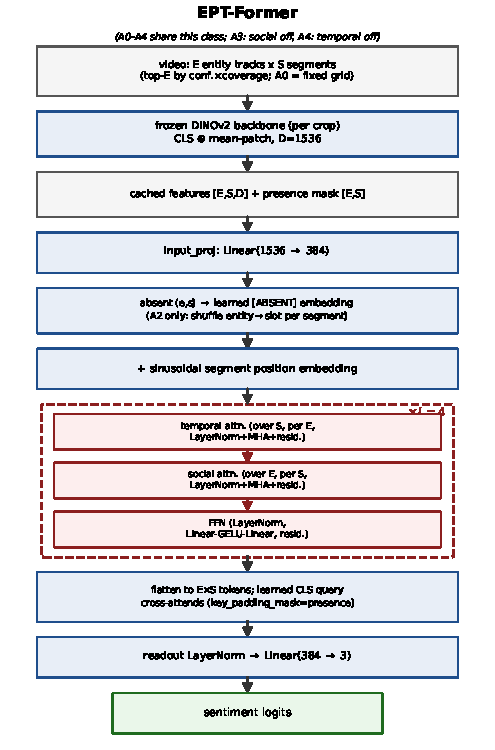
\includegraphics[width=\linewidth]{figures/fig1_architecture.pdf}
  \caption{EPT-Former forward pass. A0 and A1--A4 share this class, differing
    only in \texttt{use\_temporal}/\texttt{use\_social} and, for A0 vs.\
    A1/A3/A4, the token source (grid vs.\ entity crops).}
  \label{fig:architecture}
\end{figure}
The EPT-Former consumes the cached $[E, S, D]$ feature tensor and its
presence mask. Features are linearly projected to $d{=}384$; absent
$(e,s)$ positions are replaced with a single learned \texttt{[ABSENT]}
vector, shared across all entities and segments, before a sinusoidal
segment-position embedding is added. $L{=}4$ blocks follow, each performing
multi-head attention~\cite{vaswani2017attention} temporally (over $S$,
independently per entity), then socially (over $E$, independently per
segment), then a feed-forward layer --- 6 heads, MLP ratio 4, pre-norm
throughout. A learned CLS query
cross-attends over the flattened $E{\times}S$ token set (masked by presence)
for readout, followed by a linear classifier. Figure~\ref{fig:architecture}
diagrams the full forward pass. The whole head is
%% results/efficiency.csv: attention_stack_params column, A1 row (10652163)
10.65M parameters, independent of $E$ and $S$ (the block weights are shared
across entity and segment positions).

Two structural choices are load-bearing for the control in
\S\ref{sec:shuffle-control} and are enforced by a construction-time check,
not just a convention: \textbf{no learned per-slot identity embedding}
exists anywhere in the model (a parameter indexed by entity-slot position
would let the network recover identity from slot position alone, independent
of the token content, confounding the persistence test), and slot order is
never treated as informative --- the model is architecturally identical
whether entity $e$ occupies slot 0 or slot 5 in any given sample.

\subsection{Isolating Persistence: the Identity-Shuffle Control}
\label{sec:shuffle-control}
The question this paper asks is not ``do entity-localized tokens help'' but
specifically ``does \emph{persistent identity} across segments help, as
opposed to entity-localized cropping and a smaller token budget, which
travel with it by default.'' A1 and A0 alone cannot separate these: A0 uses
a fixed spatial grid (no entities, no persistence, a different --- typically
larger --- token count), so any A1--A0 gap is consistent with either
explanation and cannot distinguish them.

A2 isolates persistence directly: it is architecturally identical to A1 ---
same backbone features, same token count, same entity-localized crops, same
EPT-Former weights and hyperparameters --- with exactly one difference. The
entity-to-slot assignment is shuffled independently per segment, using a
deterministic per-clip seed derived from the run seed
(\texttt{shuffle\_entities\_per\_segment}, applied identically to the
feature tensor and its presence mask). The entity occupying slot 3 in
segment 1 is, in general, a different physical entity than the one occupying
slot 3 in segment 2 --- the model still receives entity-localized,
matched-budget tokens, it just can no longer track any one entity's state
across segments, because ``the token in this slot'' no longer refers to the
same tracked identity from one segment to the next. Any gap between A1 and
A2 is therefore attributable to persistence and only to persistence
(H1, \S\ref{sec:pre-registration}); any gap between A1/A2 and A0 is
attributable to entity localization and token budget, independent of
whether persistence itself does anything (H2).


\section{Experimental Setup}
%% paper/sections/pre_registration.tex
%% Draft only. Every number traced via inline LaTeX comment to its source
%% file. Covers what was planned as "Experimental Setup" (datasets, protocol,
%% conditions) plus the pre-registration discipline itself.
\label{sec:pre-registration}

\subsection{Datasets and Protocol}
\textbf{MELD}~\cite{poria2019meld}, multi-party television dialogue,
%% outputs/meld_phase1_2_summary/REPORT.md: cache/MELD_MANIFEST.json 13706 clips (train 9988, dev 1108, test 2610)
13706 clips (train 9988 / dev 1108 / test 2610), 3-class sentiment. Primary
entity budget $E{=}6$ (cached at $E_{\max}{=}8$), $S{=}4$. Identity recovery
is agglomerative face-embedding clustering (shot cuts break IoU tracking),
threshold tuned on dev only, achieving
%% outputs/meld_phase1_2_summary/REPORT.md: "Best threshold 0.55 (purity/accuracy against the character references: 62.2%..."
62.2\% clustering purity against a 6-character reference set (16.7\% chance
floor) --- imperfect identity recovery is a limitation discussed in
\S\ref{sec:limitations}, not a claim of clean tracking. MELD passed a dataset
admission procedure (\S\ref{sec:dataset-audit}) before being promoted to
primary: cross-split near-duplicate rate at 0.95 cosine similarity effectively
zero, trivial-feature-probe macro-F1
%% outputs/dataset_admission/meld/admission_report.json: trivial_probe.val_macro_f1
0.4155.

\textbf{DAiSEE}~\cite{gupta2016daisee}, single-subject e-learning webcam
video,
%% logs/GATES.md: DAiSEE 8571/8571 clips (train 5358 / val 1429 / test 1784)
8571 clips (train 5358 / val 1429 / test 1784), 4-class Engagement. Primary
entity budget locked at $E{=}1$: the detector's raw output contains multiple
candidate person-tracks per clip (background artifacts, brief ID switches),
but only the single top-confidence$\times$coverage track corresponds to the
annotated subject, so $E{=}1$ discards noise rather than signal. With one
entity slot there is no second slot to shuffle, so A2 and H1 (persistence)
are not defined for this dataset (\S\ref{sec:results}). DAiSEE's own
admission-test trivial-probe score,
%% outputs/dataset_admission/daisee/admission_report.json: trivial_probe.val_macro_f1
macro-F1 0.2177 on its subject-disjoint split, is the reference floor used to
validate the admission procedure itself (\S\ref{sec:dataset-audit}).

\textbf{OUC-CGE}~\cite{lu2025ouccge} was the originally intended primary
dataset and failed the same admission procedure; \S\ref{sec:dataset-audit}
reports the audit in full. It is retained in this paper as a rejected-dataset
case study, not as a results-table entry.

\subsection{Conditions}
A0--A5 and mask-only share the EPT-Former (\S\ref{sec:method}) or a matched
simplification of it, differing only in what tokens they receive: \textbf{A0}
--- fixed spatial grid, no entities, matched token budget; \textbf{A1} ---
full EPT, entity-localized, persistent identity (primary condition);
\textbf{A2} --- EPT with entity identity shuffled per segment
(\S\ref{sec:shuffle-control}); \textbf{A3} --- temporal attention only
(social attention disabled); \textbf{A4} --- social attention only (temporal
attention disabled); \textbf{A5} --- mean-pooled entity tokens through an
MLP, no attention at all; \textbf{mask-only} --- the presence mask alone,
with no visual features, testing whether who-is-onscreen leaks label
information by itself. A \textbf{trivial-feature probe} (linear classifier
on a single mean-pooled clip embedding, no temporal/entity/attention
structure) is reported as a standing floor in every results table, not as a
condition that went through recipe search.

\subsection{Pre-registration}
Hypotheses, decision rules, and effect-size floors were committed to
\texttt{\seqsplit{docs/DECISION\_RULES.md}} (MELD) and
\texttt{\seqsplit{docs/DECISION\_RULES\_DAISEE.md}} (DAiSEE) before any
test-split evaluation, with amendments appended and dated, never edited in
place. This is stated here as a credibility mechanism, not a formality:
every number in \S\ref{sec:results} that bears on a hypothesis was computed
after its decision criterion was frozen, not the reverse.

\textbf{H1 (persistence, MELD only).} Not defined for DAiSEE ($E{=}1$,
\S\ref{sec:method}).
\[
A1 - A2 \;\geq\; \text{EFFECT\_FLOOR} \quad \text{(macro-F1)}
\]

\textbf{H2 (entity structure).} MELD uses macro-F1 directly; DAiSEE
restricts macro-F1 to classes 1--3 (see below).
\[
A1 - A0 \;\geq\; \text{EFFECT\_FLOOR} \quad \text{(macro-F1)}
\]

\textbf{Decision rule (MELD, three branches).} A branch fires only if both
the point estimate clears \texttt{EFFECT\_FLOOR} \emph{and} a paired
bootstrap over test items (10{,}000 resamples) gives a 95\% CI excluding
zero.
\begin{align*}
\text{(a)}&\quad A1 - A2 \geq \text{EFFECT\_FLOOR} \\
\text{(b)}&\quad |A1{-}A2| < \text{EFFECT\_FLOOR} \ \text{and H2 supported} \\
\text{(c)}&\quad A1 < A2 - \text{EFFECT\_FLOOR}
\end{align*}
Branch (a): persistence is the mechanism. Branch (b): entity localization
and token budget matter, persistence does not. Branch (c): hypothesis
refuted.

\textbf{Decision rule (DAiSEE, H2 only, two conditions).} Same paired
requirement as above.
\begin{align*}
\text{(a)}&\quad \text{margin} \geq \text{EFFECT\_FLOOR} \\
\text{(b)}&\quad |\text{margin}| < \text{EFFECT\_FLOOR} \\
\text{(c)}&\quad \text{margin} < -\text{EFFECT\_FLOOR}
\end{align*}
Branch (a): supported. Branch (b): null/underpowered. Branch (c): reversed.

\textbf{Effect floors, computed blind.} For each dataset, seed-level and
item-level macro-F1 variance was bootstrapped on dev/val \emph{before}
inspecting which condition scored higher --- only dispersion was ever
recorded --- then \texttt{EFFECT\_FLOOR} was set to twice the pooled SE,
floored at $0.02$ and rounded up:
\[
\text{EFFECT\_FLOOR} = \max(0.02,\ 2\,\text{SE})
\]
MELD's pooled SE was $0.0170$, giving $\text{EFFECT\_FLOOR}=0.04$
%% docs/DECISION_RULES.md 2026-08-15 amendment ("Effect floor computed"): pooled_SE=0.0170
%% commit a6d19a8 (procedure fixed) / 8c156a9 (floor computed)
(\texttt{a6d19a8}/\texttt{8c156a9}). DAiSEE's pooled SE was $0.0138$, giving
$\text{EFFECT\_FLOOR}=0.03$
%% docs/DECISION_RULES_DAISEE.md 2026-08-15 amendment: pooled_SE=0.0138
%% commit 00dcc1d (pre-registration) / 7c2c0d0 (floor computed)
(\texttt{00dcc1d}/\texttt{7c2c0d0}). Both studies are, by this procedure,
explicitly underpowered for the originally-hoped 0.02 margin --- stated in
the amendment before either floor was used to evaluate anything, not
discovered after the fact.

\textbf{DAiSEE primary-metric amendment.}
%% commit 347115b, committed before Phase 4 ran
Committed before DAiSEE's test evaluation (\texttt{347115b}), the primary
metric for DAiSEE's H2 was restricted to macro-F1 over classes 1--3, excluding
class 0 from the average (reported separately as a raw count and raw F1 in
every table, never dropped silently). Class 0 has
%% docs/DECISION_RULES_DAISEE.md: test distribution {0:4,...}
4 test clips --- too few to support a macro-averaged claim --- and scored
%% docs/LOCKED_RECIPE_DAISEE.md: class 0 F1 == 0.000 in 9 of 16 grid runs, val
0.000 F1 in 9 of 16 dev-search grid points despite 23 val clips to calibrate
against. \texttt{EFFECT\_FLOOR} was explicitly \emph{not} recomputed for the
new metric, to avoid letting the threshold move with information gathered
after the original blind bootstrap. The amendment used only val-split
behavior and test-set item counts; no test-split performance had been
observed at the time it was written.


\section{Results}
%% paper/sections/results.tex
%% Draft only. All three pre-registered structural hypotheses are null; no
%% hedging toward a positive reading anywhere below. Every number traced via
%% inline LaTeX comment.
\label{sec:results}

\subsection{Structural Hypotheses: All Three Null}
Three pre-registered hypotheses were evaluated against locked recipes, test
touched exactly once per condition/seed
(\S\ref{sec:pre-registration}). All three are null.

\textbf{H1, MELD (persistence).}
%% outputs/meld_phase4_statistics.json: h1_persistence.mean_margin, ci_low, ci_high
$A1 - A2 = 0.0340$, 95\% CI $[0.0203, 0.0480]$. The CI excludes zero, but the
point estimate is below $\text{EFFECT\_FLOOR}{=}0.04$. \textbf{Not
supported.} Per the frozen decision rule, this is reported as underpowered,
not as evidence that persistence has no effect.

\textbf{H2, MELD (entity structure).}
%% outputs/meld_phase4_statistics.json: h2_entity_structure.mean_margin, ci_low, ci_high
$A1 - A0 = 0.0315$, 95\% CI $[0.0159, 0.0470]$. Same pattern: CI excludes
zero, point estimate below the floor. \textbf{Not supported.} With neither H1
nor H2 clearing $\text{EFFECT\_FLOOR}$, none of the three branches in the
MELD decision rule fire
%% outputs/meld_phase4_statistics.json: decision.branch == null
--- reported as such, not forced into the nearest branch.

\textbf{H2, DAiSEE (replication).}
%% outputs/daisee_phase4_statistics.json: h2_item_paired_bootstrap.mean_margin, ci_low, ci_high
$A1 - A0 = 0.0037$, 95\% CI $[-0.0199, 0.0264]$, primary metric (macro-F1,
classes 1--3, \S\ref{sec:pre-registration}). The CI includes zero.
\textbf{Not supported} --- branch (b), null/underpowered, per the frozen
rule
%% outputs/daisee_phase4_statistics.json: decision.branch == "b"
.

\textbf{These are two different flavors of null, and the difference matters
for how they're read.} MELD's H1 and H2 margins are positive with CIs that
exclude zero --- a real, non-noise signal that simply does not clear the
pre-registered bar. DAiSEE's H2 margin is indistinguishable from zero by
every measure computed (\S\ref{sec:sensitivity}). MELD's H2 (0.0315) does
not replicate as DAiSEE's H2 (0.0037): the same structural comparison,
entity-localized tokens against a matched-budget spatial grid, produces a
detectable-but-underpowered gap on multi-party television video and no
detectable gap at all on single-subject webcam video. We report this as a
\textbf{failure to replicate}, not as a stronger MELD finding standing
uncontested.

One \emph{post hoc, untested} hypothesis for the divergence, offered here
explicitly as such and not fit to any data beyond what is already reported:
DAiSEE's $E{=}1$ crop is a single dominant-subject region that likely already
covers most of the frame's informative content, since webcam framing
centers the subject by construction; MELD's multi-party wide shots contain
substantially more frame area outside any one speaker, so entity-localized
cropping there discards more distractor content than it does on DAiSEE. If
this is right, the entity-vs-grid gap should scale with how much of the
frame a matched-budget grid wastes on non-entity content --- a claim this
paper does not test.

\subsection{Purity-Stratified Secondary Analysis (MELD)}
Pre-registered before computation, secondary to the branch decision above:
%% outputs/meld_phase4_purity_stratified.json: tercile_p33, tercile_p67, tercile_counts
MELD test clips were split into purity terciles (silhouette-score-based
identity-clustering quality, cutpoints $0.8008$/$0.9067$, 870 clips each) and
H1's margin recomputed within each. If persistence's pooled null reflected
imperfect identity recovery (\S\ref{sec:pre-registration}'s 62.2\% clustering
purity) rather than a true absence of effect, the margin should grow
monotonically with purity. It does not:
%% outputs/meld_phase4_purity_stratified.json: margins_low_mid_high, monotone
margins are $0.0377$ (low purity), $0.0264$ (mid), $0.0389$ (high) --- not
monotone. This argues against ``identity wasn't recovered well enough to
tell'' as the explanation for the pooled null, without resolving it into a
positive finding either.

\subsection{Sensitivity and Robustness}
\label{sec:sensitivity}
\begin{figure}[t]
  \centering
  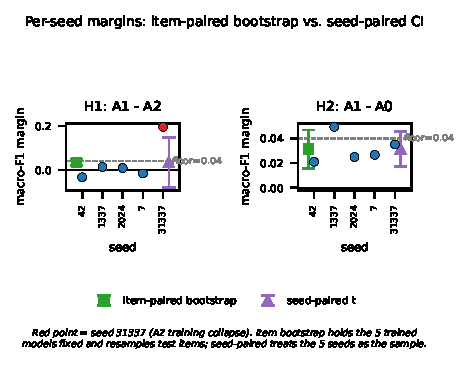
\includegraphics[width=\linewidth]{figures/fig4_seed_margin_divergence.pdf}
  \caption{Per-seed H1/H2 margins (MELD), item-paired bootstrap vs.\
    seed-paired $t$ interval. Seed 31337 (red, H1 panel) is A2's training
    collapse; the two interval estimates diverge for H1 and agree for H2.}
  \label{fig:seed-margin}
\end{figure}
\textbf{Leave-one-seed-out (MELD).} Dropping seed 31337 --- which collapsed
during A2 training (dev macro-F1 falling to majority-class level in the
final two epochs, visible in both train and dev curves at that seed) ---
flips H1's margin sign
%% outputs/meld_phase4_posthoc_analysis.json: leave_one_out_h1, seed 31337 entry
(from $+0.034$ pooled to $-0.006$ with that seed excluded); dropping any of
the other four seeds individually keeps H1 close to or above $0.04$
%% outputs/meld_phase4_posthoc_analysis.json: leave_one_out_h1, all five drop-one entries (0.0390-0.0508 excluding the 31337 drop)
(0.0390--0.0508; three of the four stay above the floor, dropping seed 1337
alone brings it to 0.0390, just under). H2 is stable under every
leave-one-out fold. This is diagnostic, not a revision: the pre-registered
5-seed result stands.

\textbf{Item-paired vs.\ seed-paired tests diverge for H1, agree for H2
(MELD).} A seed-paired $t$-test on H1's five per-seed margins gives
%% outputs/meld_phase4_posthoc_analysis.json: seed_paired_h1.paired_t_p, wilcoxon_p
$p{=}0.457$ (Wilcoxon $p{=}1.0$) --- no significant effect --- against the
item-paired bootstrap's zero-excluding CI above. For H2, the seed-paired test
gives
%% outputs/meld_phase4_posthoc_analysis.json: seed_paired_h2.paired_t_p, wilcoxon_p
$p{=}0.0034$ (Wilcoxon $p{=}0.0625$, the smallest attainable at $n{=}5$),
agreeing with the item-paired result. The divergence for H1 is explained by
what each test conditions on: the item-paired bootstrap holds the five
already-trained models fixed and asks only whether the margin survives
resampling test items, so a single collapsed seed's degenerate predictions
stay degenerate in every resample; the seed-paired test treats the five
per-seed margins as the sample, so that same collapse dominates the
between-seed variance directly. H2 has no comparable outlier seed, and the
two tests agree.

\textbf{Item-paired and seed-paired agree for DAiSEE's H2.} Paired $t$
%% outputs/daisee_phase4_statistics.json: h2_seed_paired.paired_t_p, wilcoxon_p
$p{=}0.793$, Wilcoxon $p{=}0.8125$ --- both consistent with the item-paired
CI including zero. No seed behaved like MELD's 31337; this null is not an
artifact of one bad run.

\subsection{Ablations}
%% results/summary.csv: A3, A4, A5, mask_only rows (macro_f1_mean +/- macro_f1_std)
A3 (temporal-only) reaches $0.4032{\pm}0.0431$ and A4 (social-only) reaches
$0.4111{\pm}0.0311$, both close to A1's $0.4040{\pm}0.0077$
(\S\ref{sec:pre-registration}'s primary condition) --- neither attention axis
alone is doing dramatically more or less than the combination. A5
(mean-pooled entities, no attention at all,
%% results/summary.csv: A5 row
$0.3901{\pm}0.0081$) is within noise of A0
%% results/summary.csv: A0 row
($0.3725{\pm}0.0092$) and not far below A1, consistent with
\S\ref{sec:efficiency}'s finding that attention structure contributes little
compute and, on this evidence, not dramatically more accuracy either.
Mask-only
%% results/summary.csv: mask_only row
($0.2459{\pm}0.0021$) fails to clear the trivial-feature-probe floor
($0.3648$, \S\ref{sec:pre-registration}) at every seed --- who is on screen,
alone, does not predict sentiment on MELD.

\subsection{Efficiency}
\label{sec:efficiency}
\begin{figure}[t]
  \centering
  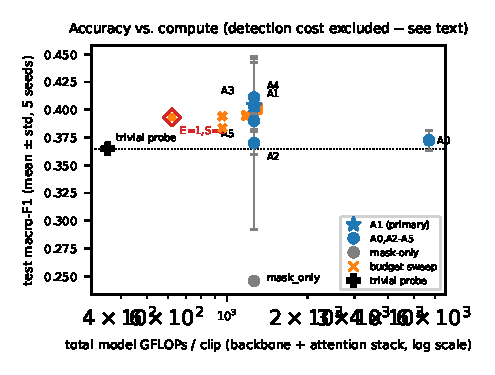
\includegraphics[width=\linewidth]{figures/fig3_pareto_gflops.pdf}
  \caption{Accuracy vs.\ latency by hardware regime (MELD). No panel mixes
    GPU- and CPU-measured numbers. Regime A (GPU-only) is not measured:
%% outputs/meld_phase6_gpu_detection_attempt.json: root_cause
    \texttt{onnxruntime-gpu} 1.28.0's prebuilt wheel requires CUDA 13's
    \texttt{libcublasLt.so.13}, but this environment provides only CUDA
    12.8 runtime libraries (matching the CUDA-12.8-pinned PyTorch build used
    throughout, itself pinned for Blackwell/sm\_120 support); the two are
    mutually incompatible here, so no GPU-only detection latency exists to
    plot (\S\ref{sec:efficiency}).}
  \label{fig:pareto}
\end{figure}
\textbf{Cost lives in encoding, not fusion.} EPT-Former's own attention
--- temporal, social, and CLS-readout combined --- is
%% results/efficiency_breakdown.csv: A1 row, fusion_attention_pct_of_total
$0.0192\%$ of A1's total per-clip compute; across every condition and every
budget-sweep cell it stays under $0.03\%$
%% outputs/meld_phase6_gflops_breakdown.json: condition_rows / budget_sweep_rows, fusion_attention_pct_of_grand_total range
. The frozen DINOv2~\cite{oquab2023dinov2} encoder --- itself attention-based, applied once per
crop to far more patch tokens than EPT-Former ever fuses --- is essentially
the entire cost. This is not a claim that attention is intrinsically cheap;
it is a claim about token count at each stage. The original motivation for
this line of work (reducing attention cost by giving it fewer, better
tokens) targets a cost term that turns out to be minor.

\textbf{The encoder-cost reduction itself is real and unconditional.}
Entity-localized cropping cuts encoder cost
%% outputs/meld_phase6_gflops_breakdown.json: encoder_reduction_a0_to_a1
$4.53\times$ relative to the spatial grid
%% results/efficiency_breakdown.csv: A0, A1 rows, encoder_gflops
($5709.7 \to 1261.0$ GFLOPs/clip, A0$\to$A1) --- a deterministic architectural
fact, not a noisy estimate. The macro-F1 difference that accompanies it on
MELD is the same $0.0315$ reported as H2 above: positive, CI excluding zero,
below the pre-registered floor. We do not double-count it as a second,
independent positive finding here --- A0 costs $4.53\times$ more encoder
compute than A1 for an accuracy difference this paper's own pre-registered
criterion does not certify as established.

\textbf{End-to-end cost depends on which hardware regime is asked about, and
the honest answer is a range, not a number.} Detection could not be measured
on GPU: \texttt{onnxruntime-gpu} 1.28.0's CUDA provider failed to load
(\texttt{libcublasLt.so.13} missing --- this build targets CUDA 13 against an
environment pinned to CUDA 12.8 for Blackwell support), so the GPU-only
regime is reported as unavailable, not estimated
%% outputs/meld_phase6_gpu_detection_attempt.json: root_cause; outputs/meld_phase6_regimes.json: A_gpu_only.available=false
. Three internally-consistent regimes were measured instead. CPU-only, both
model and detection at 1 thread: A1 costs
%% outputs/meld_phase6_regimes.json: B_cpu_only_threads1.A1_vs_A0_ratio
$0.32\times$ A0 (A1 is cheaper). CPU-only, both at 60 threads
(model: intra-op; detection: 60-way process throughput --- different
parallelism mechanisms spending the same thread budget, not directly
comparable mechanisms): A1 costs
%% outputs/meld_phase6_regimes.json: B_cpu_only_threads60.A1_vs_A0_ratio
$0.23\times$ A0. A stated-assumption ``realistic deployment'' split (model on
GPU, detection on a CPU pool at 60-way throughput): A1 costs
%% outputs/meld_phase6_regimes.json: C_realistic_deployment.A1_vs_A0_ratio
$7.49\times$ A0, since A0 needs no detector at all. \textbf{The range,
$0.23\times$--$7.49\times$, is the honest result} --- token reduction
reliably cuts the encoder term, but whether that makes the full pipeline
cheaper or more expensive than the grid baseline depends entirely on where
detection is run and how its cost is amortized, not on any single number.

\textbf{The budget sweep's cheapest useful point.}
%% outputs/meld_phase4_budget_sweep_summary.json (E=1,S=2 mean, computed from results); A1's own summary.csv row
$E{=}1,S{=}2$ (2 tokens) reaches macro-F1 $0.3932$, $97.3\%$ of A1's own
$E{=}6,S{=}4$ result ($0.4040$), at
%% results/efficiency_budget_sweep.csv: e=1,s=2 row, total_model_gflops_per_clip
$621.5$ GFLOPs/clip against A1's $1261.5$. Every one of the 10 budget-sweep
cells' CIs exclude the trivial-feature probe; $E{=}1,S{=}2$ is the smallest
by token count that does
%% outputs/meld_phase4_posthoc_analysis.json: smallest_excluding_probe (e=1,s=2, t_p=0.00031)
.


\section{Discussion and Limitations}
%% paper/sections/discussion.tex
%% Draft only. Limitations get their own subsection, six specific items.
\label{sec:discussion}

Three pre-registered structural hypotheses were tested under a decision
rule and effect-size floor frozen before any test-split evaluation
(\S\ref{sec:pre-registration}), and all three came back null
(\S\ref{sec:results}). MELD's H1 and H2 are the underpowered-but-real flavor
of null --- positive margins, confidence intervals excluding zero, both
still short of the pre-registered bar; DAiSEE's H2 replication is the
indistinguishable-from-zero flavor, agreeing across item-paired and
seed-paired tests alike. Read together, the honest summary is not
``persistence doesn't matter'' or ``entity structure doesn't matter'' ---
this study's power does not license either claim --- but that the specific,
falsifiable version of both claims this paper pre-registered did not survive
contact with a locked test set, on either dataset. The identity-shuffle
control (\S\ref{sec:shuffle-control}) did the job it was designed to do: it
gave persistence a real chance to show a distinguishable effect against
entity-localized cropping and token budget, under conditions where the
architecture, features, and everything else were held fixed, and the effect
it isolated did not clear the bar set for it in advance.

The efficiency results (\S\ref{sec:efficiency}) are not a consolation
finding dressed up to offset the null hypotheses --- they are a separate,
narrower claim about where compute goes, and they hold regardless of how H1
and H2 came out. Entity-localized cropping cuts encoder cost by $4.53\times$
unconditionally; end-to-end cost relative to a grid baseline depends on
hardware placement in a way that spans a $0.23\times$--$7.49\times$ range,
not a single number; and the attention mechanism this paper's architecture
is built around turns out to be a rounding error in the compute budget
compared to the frozen encoder it sits on top of. If token-count-driven
efficiency work in this space wants to target the dominant cost term, that
term is per-crop encoding, not fusion attention.

\subsection{Limitations}
\label{sec:limitations}

\textbf{Frozen backbone, no fine-tuning.} Every condition in this paper,
including the grid baseline, consumes the same frozen DINOv2~\cite{oquab2023dinov2} features
(\S\ref{sec:method}). This is deliberate --- it is what makes the matched-
feature comparison possible --- but it means no result here speaks to
whether entity-persistent tokenization would change what an end-to-end
fine-tuned encoder learns, only to what a fixed, off-the-shelf visual
representation supports downstream.

\textbf{One architecture family.} EPT-Former is a standard multi-head-attention
transformer applied to a differently-defined token stream
(\S\ref{sec:method}); this paper does not test whether the same entity-
persistent tokens would behave differently under a state-space or
convolutional fusion mechanism, only under attention.

\textbf{MELD's identity recovery is imperfect.}
%% outputs/meld_phase1_2_summary/REPORT.md: 62.2% purity, 16.7% chance floor
Clustering purity against a 6-character reference set is 62.2\% (16.7\%
chance floor) --- well above chance but far from clean tracking. The
purity-stratified analysis (\S\ref{sec:results}) argues the pooled H1 null
is not simply an artifact of this, but it cannot rule out that better
identity recovery would move the result; it can only show the result is not
obviously monotone in purity as measured.

\textbf{DAiSEE's $E{=}1$ degeneracy.} DAiSEE's primary condition has exactly
one entity slot (\S\ref{sec:pre-registration}), so A2 and H1 do not exist for
it by construction. The DAiSEE replication tests H2 only; it says nothing
about persistence on single-subject video, because there is no second slot
for identity to persist across.

\textbf{GPU detection cost is unmeasured, not zero.} Every end-to-end cost
regime that involves detection uses CPU-measured detection latency
(\S\ref{sec:efficiency}); the GPU-only regime could not be measured due to a
CUDA-version mismatch in the available \texttt{onnxruntime-gpu} build, not
because GPU detection is expected to be free. A working GPU detection
measurement could shift the low end of the reported ratio range.

\textbf{OUC-CGE's effective sample size is unrecoverable.} The dataset-audit
connected-components analysis
%% outputs/phase3_5_audit/TRACK1_TRACK2_REPORT.md sec.4: "plausibly in the tens, not the thousands"
(\S\ref{sec:dataset-audit}) finds the corpus's effective number of
independent, exchangeable recording units is plausibly in the tens, not the
thousands implied by its 7700-clip count, but that no similarity threshold
recovers a trustworthy estimate of the true number. This is why OUC-CGE is
reported only as a case study, never as a results-table entry: not just its
split, but its usable sample size, is not something this paper's methods can
put a reliable number on.


\section{Conclusion}
%% paper/sections/conclusion.tex
%% Draft only. Brief, consistent with the all-null framing throughout.
\label{sec:conclusion}

This paper tested whether giving a video transformer tokens with a genuine
persistent referent changes what it learns, using a control designed to
isolate persistence from the entity-localized cropping and reduced token
budget that ordinarily travel with it. Under a decision rule and effect-size
floor frozen before any test-split evaluation, all three pre-registered
structural hypotheses came back null: MELD's persistence and entity-structure
margins are positive with confidence intervals excluding zero but short of
the pre-registered floor, and the entity-structure comparison's replication
on DAiSEE is indistinguishable from zero outright
(\S\ref{sec:results}--\ref{sec:discussion}). We report this as the finding,
not as a setback to be explained away: a pre-registered null, arrived at
through a control built specifically to make the positive result easy to
see if it were there, is evidence about the hypothesis, not an absence of
result.

Separately, and unconditionally on how the hypotheses resolved, entity-
localized cropping cuts per-crop encoder cost by $4.53\times$, the attention
mechanism this architecture is built around accounts for a fraction of a
percent of total compute, and the end-to-end cost of trading a spatial grid
for tracked entities depends on where detection is run --- a
$0.23\times$--$7.49\times$ range, not a single favorable number
(\S\ref{sec:efficiency}). Together with the dataset-admission procedure this
work produced as a reusable artifact (\S\ref{sec:dataset-audit}), the
contribution of this paper is less a positive architectural result than a
demonstration of what a fully pre-registered, matched-feature, cost-honest
evaluation of an intuitive idea actually looks like when the idea does not
clear its own bar.


\section*{Ethics Statement}
OUC-CGE~\cite{lu2025ouccge} and MELD~\cite{poria2019meld} are used under
their respective stated release terms (OUC-CGE: CC-BY-4.0). The dataset
audit in \S\ref{sec:dataset-audit} concerns split-protocol properties ---
near-duplicate content assigned across train/val/test partitions --- not
individuals, and no attempt was made to identify, track, or re-identify any
person appearing in either corpus beyond the anonymized entity-tracking
already required by this paper's own method. The OUC-CGE leakage finding
reported in \S\ref{sec:dataset-audit} is a property of the released
partition, not of the underlying recordings, their collection, or their
authors.

\begin{acks}
%% Omit entirely in anonymous mode — the acks environment handles this automatically.
\end{acks}

\bibliographystyle{ACM-Reference-Format}
\bibliography{refs}

\end{document}
